\documentclass[11pt]{article}

\usepackage[a4paper,margin=22mm]{geometry}
\usepackage[utf8]{inputenc}
\usepackage[T1]{fontenc}
\usepackage{amsmath,amssymb}
\usepackage{graphicx}
\usepackage{booktabs}
\usepackage{longtable}
\usepackage{xcolor}
\usepackage{hyperref}

\hypersetup{
  colorlinks=true,
  linkcolor=blue!55!black,
  urlcolor=blue!65!black
}
\setlength{\parindent}{0pt}
\setlength{\parskip}{0.65em}
\renewcommand{\arraystretch}{1.18}

\newcommand{\infid}{1-F}
\newcommand{\pPar}{p_{\parallel}}
\newcommand{\Om}{\Omega}
\newcommand{\dOm}{\delta\Omega}
\newcommand{\target}{10^{-5}}
\newcommand{\Hgate}{H_{\mathrm{gate}}}
\newcommand{\Hess}{\mathcal{H}_{F}}
\newcommand{\figReading}[1]{\paragraph{How to read it.}#1}
\newcommand{\figMeaning}[1]{\paragraph{What it means.}#1}
\newcommand{\figCaution}[1]{\paragraph{Important caution.}#1}

\title{Reading Notes for the Closed-Loop Hessian Failure Figures}
\author{Extension study based on arXiv:2606.05060v1}
\date{28 July 2026}

\begin{document}
\maketitle

\begin{abstract}
These notes explain the nine figures generated in the extension study of
low-rank-Hessian closed-loop calibration for a neutral-atom controlled-$Z$
(CZ) gate.  The aim is not only to say whether a run succeeds, but to
distinguish four possible causes of failure: a distortion that is too large
for the quadratic model, rotation of the sensitive control subspace,
measurement/fit noise, and a new physical error channel that is absent from
the nominal Hessian.
\end{abstract}

\tableofcontents
\newpage

\section{Minimal background}

\subsection{Complete symbol and label dictionary}

This section defines the notation used in the figures and in the explanations
below.  In particular, $\Om_c$ and $\Om$ are different objects:
$\Om_c(t)$ is the full complex, time-dependent control, whereas $\Om$ is its
reference magnitude and the frequency unit used on several axes.

\subsubsection{Pulse, time, and quantum states}

\begin{longtable}{p{0.20\textwidth}p{0.71\textwidth}}
\toprule
Symbol or label & Meaning\\
\midrule
\endhead
$t$ & Physical time during one gate pulse.\\
$T$ & Total gate duration.  Therefore $t/T$ is normalized time, running from
0 at the pulse start to 1 at the pulse end.\\
$\Om_c(t)$ & Complex control Rabi frequency applied to the atoms.  Its real
and imaginary parts are the two Cartesian control quadratures.\\
$\Om$ & Positive reference Rabi-frequency magnitude.  For the analytical
pulse $|\Om_c(t)|=\Om$.  It also sets the units of $\omega$, detuning, and
Hamiltonian-perturbation strength.\\
$|\Om_c|/\Om$ & Pulse magnitude divided by the reference magnitude.  A value
of 1 means no amplitude modulation.\\
$\phi(t)$ & Time-dependent phase of the complex control:
$\Om_c(t)=|\Om_c(t)|e^{i\phi(t)}$.\\
$A$ & Dimensionless amplitude of the phase modulation.\\
$\omega$ & Angular frequency of the phase modulation, measured here in units
of $\Om$.\\
$\phi_0$ & Phase offset inside the cosine modulation.\\
$\delta_0$ & Optional linear phase-ramp coefficient in
$\phi(t)=A\cos(\omega t-\phi_0)+\delta_0t$.  It is set to zero in this run.\\
$i$ & Imaginary unit, $i^2=-1$.  In a subscript such as $\lambda_i$ or
$v_i$, $i$ instead denotes the mode number.\\
$\pi$ & Circle constant.  A phase of $\pi$ radians is $180^\circ$.\\
$|0\rangle,|1\rangle$ & The two computational states of one atom.\\
$|r\rangle$ & The Rydberg excited state of one atom.\\
$|01\rangle,|10\rangle,|11\rangle$ & Two-atom computational basis states.
For example, $|01\rangle=|0\rangle\otimes|1\rangle$.\\
$|0r\rangle,|r0\rangle$ & Single-Rydberg leakage partners of
$|01\rangle$ and $|10\rangle$.\\
$|W\rangle$ & Symmetric blockaded Rydberg state
$\left(|r1\rangle+|1r\rangle\right)/\sqrt{2}$ coupled to $|11\rangle$.\\
$\langle a|b\rangle$ & Inner product of states $|a\rangle$ and $|b\rangle$.
An expression $|a\rangle\langle b|$ maps $|b\rangle$ to $|a\rangle$.\\
$\mathrm{h.c.}$ & Hermitian conjugate; it adds the reverse couplings required
to make the Hamiltonian Hermitian.\\
CZ & Controlled-$Z$ gate: ideally only $|11\rangle$ acquires an additional
phase of $\pi$, up to correctable single-qubit $Z$ phases.\\
\bottomrule
\end{longtable}

\subsubsection{Waveform distortion and Hessian geometry}

\begin{longtable}{p{0.20\textwidth}p{0.71\textwidth}}
\toprule
Symbol or label & Meaning\\
\midrule
\endhead
$\Om_0(t)$ & Nominal analytical control waveform before an artificial
distortion is added.\\
$\dOm(t)$ & Complex waveform distortion:
$\dOm(t)=\Om_c(t)-\Om_0(t)$.\\
$\dOm$ without $(t)$ & The real control vector obtained by stacking
$\operatorname{Re}\dOm$ and $\operatorname{Im}\dOm$ at all time bins.  Its
length is $2N$.\\
$\operatorname{Re}(z)$, $\operatorname{Im}(z)$ & Real and imaginary parts of
a complex quantity $z$.\\
$|z|$ & Absolute value for a real number or magnitude for a complex number.\\
$\|x\|$ & Euclidean norm of a vector $x$; $\|x\|^2$ is its total squared
amplitude.\\
$N$ & Number of time bins, $N=256$ in this run.\\
$\eta$ & Relative root-mean-square waveform distortion,
$\eta=\sqrt{\int|\dOm|^2dt/\int|\Om_0|^2dt}$.  It measures waveform size,
not gate infidelity.\\
$\Hess$ & Leading fidelity Hessian in the real waveform coordinates.  It is
the quadratic sensitivity matrix of the five first-order error channels.\\
$\dOm^{\mathsf T}$ & Transpose of the real distortion vector.  Hence
$\dOm^{\mathsf T}\Hess\dOm/2$ is a scalar predicted infidelity.\\
$O(\|\dOm\|^3)$ & Terms cubic and higher in distortion magnitude that are
discarded by the leading quadratic approximation.\\
$\lambda_i$ & $i$th Hessian eigenvalue, ordered from largest to smallest.  A
larger value means stronger local sensitivity along that eigenvector.\\
$\lambda_1$ & Largest Hessian eigenvalue, used to normalize the spectrum.\\
$|\lambda_i|/\lambda_1$ & Relative magnitude of Hessian mode $i$.  The
declared active-rank threshold is $10^{-8}$.\\
$v_i$ & Normalized eigenvector associated with $\lambda_i$; it is one
waveform direction scanned by the closed loop.\\
$\operatorname{Re}(v_i)$, $\operatorname{Im}(v_i)$ & Real and imaginary
control quadratures of eigenvector $v_i$.\\
$\sqrt{N}\,v_i$ & Plotting rescaling of a unit-norm discrete eigenvector.
Multiplication by $\sqrt N$ makes typical curve values order one; it does not
change the direction.\\
$P_{\Hess}$ & Orthogonal projector onto the five-dimensional space spanned by
$v_1,\ldots,v_5$.\\
$\pPar$ & Fraction of distortion power in that five-dimensional space:
$\pPar=\|P_{\Hess}\dOm\|^2/\|\dOm\|^2$.\\
principal space & Span of the five active nominal Hessian eigenvectors.\\
null space & All nominal waveform directions orthogonal to that principal
space; their leading quadratic prediction is zero.\\
principal angle & Standard angle comparing two subspaces.  Zero degrees means
alignment; 90 degrees means that at least one direction is orthogonal.\\
singular overlap & Singular value of the overlap matrix between two
orthonormal subspace bases.  One means perfect retention and zero means a
lost direction.\\
\bottomrule
\end{longtable}

\subsubsection{Fidelity, leakage, phase, and noise}

\begin{longtable}{p{0.20\textwidth}p{0.71\textwidth}}
\toprule
Symbol or label & Meaning\\
\midrule
\endhead
$F$ & Average CZ gate fidelity after removing freely correctable local
single-qubit $Z$ phases.  An ideal gate has $F=1$.\\
$\infid$ & Gate infidelity.  Smaller is better; success is declared when
$\infid\leq\target$.\\
$10^{-5}$ & The chosen success threshold, corresponding to fidelity
$F\geq0.99999$.\\
$P_{\mathrm{leak},01}$ & Probability that population starting in the
$|01\rangle$ sector finishes outside its computational state.\\
$P_{\mathrm{leak},11}$ & Corresponding leakage probability for the
$|11\rangle$ blockaded sector.\\
$a_{01},a_{10},a_{11}$ & Complex return amplitudes of the three nontrivial
computational sectors after the pulse.  Their magnitudes encode survival and
their arguments encode phase.\\
$\arg(z)$ & Complex phase (argument) of $z$, expressed in radians.\\
$\theta_{\mathrm{CZ}}$ & Nonlinear two-qubit phase
$\arg(a_{11})-\arg(a_{01})-\arg(a_{10})$; the CZ target is $\pi$ modulo
$2\pi$.\\
$\delta\theta$ & Wrapped error of $\theta_{\mathrm{CZ}}$ relative to $\pi$.\\
$\delta\theta^2/5$ & Nonlinear-phase proxy used for the green bars in
Figure~6.  It is a diagnostic scale, not an independently additive
probability.\\
$\sigma_F$ & Standard deviation of independent additive Gaussian noise placed
on each scalar fidelity evaluation in Figure~7.\\
non-positive fit & A seven-point quadratic line fit whose fitted curvature is
zero or negative; this signals an unresolved or non-convex local minimum.\\
channel diagnostic & A leakage probability or phase-error proxy plotted to
show which physical error remains.\\
\bottomrule
\end{longtable}

\subsubsection{Algorithmic labels appearing on the plots}

\begin{longtable}{p{0.24\textwidth}p{0.67\textwidth}}
\toprule
Plot label & Meaning\\
\midrule
\endhead
mode & One normalized Hessian eigenvector $v_i$.  There are five scanned
modes.\\
accepted mode update & One completed one-dimensional scan followed by the
applied coefficient update along one mode.  Five updates make one complete
cycle unless the success target stops the run early.\\
seven-point fit & Seven symmetric coefficient samples along one mode,
followed by a bounded quadratic fit and an update to its fitted minimum.\\
exact line minimum & A simulation-only oracle that numerically minimizes the
true propagated infidelity along one mode.\\
exact propagation & Direct unitary propagation of the stated Hamiltonian,
without truncating the time dynamics to the Hessian approximation.\\
initial/final & Value before the first closed-loop update and after the last
accepted update, respectively.\\
before loop/after loop & Same meaning as initial/final in Figure~9.\\
success fraction & Number of random seeds reaching the target divided by ten
trials in that scan cell.\\
seed & Integer identifying one reproducible random smooth distortion shape.\\
cycle & One pass through the five nominal Hessian directions.\\
residual floor & Final infidelity remains above $\target$ after the allowed
eight cycles.\\
perturbation strength$/\Om$ & Hamiltonian-error amplitude divided by the
reference Rabi frequency; for example, 0.1 means $0.1\Om$.\\
degrees & Unit of the principal angle; $180^\circ=\pi$ radians.\\
rank threshold & Relative-eigenvalue cutoff
$|\lambda_i|/\lambda_1>10^{-8}$ used to count active Hessian modes.\\
logarithmic axis & Equal vertical distances represent equal multiplicative
ratios.  Moving by one decade changes a value by a factor of ten.\\
median & Middle value of the ten seeds after sorting; it is less sensitive to
an extreme seed than the arithmetic mean.\\
90th-percentile shading & In Figure~4, the shaded region runs from the median
to a value exceeded by only about 10\% of seeds.\\
relative model discrepancy & In Figure~4,
$|E_{\mathrm{nonlinear}}-E_{\mathrm{quad}}|/
\max(E_{\mathrm{nonlinear}},10^{-10})$.\\
\bottomrule
\end{longtable}

\subsection{Model and fidelity target}

The calculation uses the perfect-blockade, symmetric two-atom model
\begin{equation}
\Hgate(t)=\frac{1}{2}\left\{
\Om_c(t)\left[
|0r\rangle\langle 01|
+|r0\rangle\langle 10|
+\sqrt{2}\,|W\rangle\langle 11|
\right]+\mathrm{h.c.}\right\}.
\end{equation}
The analytical control has constant magnitude and time-dependent phase,
\begin{equation}
\Om_c(t)=\Om e^{i\phi(t)},\qquad
\phi(t)=A\cos(\omega t-\phi_0)+\delta_0t,
\end{equation}
with the published rounded parameters
$A=2\pi(0.1122)$, $\omega=1.0431\Om$, $\phi_0=-0.7318$, and
$\delta_0=0$, with $\Om T/(2\pi)=1.215$.

The plotted error is the average gate infidelity $\infid$.  A calibration
trial is called successful if
\begin{equation}
\infid\leq\target
\end{equation}
within eight complete cycles.  One cycle scans all five nominal Hessian
directions.

\subsection{Why there are five directions}

Close to an ideal pulse, the gate error is approximated by
\begin{equation}
\infid
=\frac{1}{2}\dOm^{\mathsf T}\Hess\,\dOm
+O(\|\dOm\|^3).
\end{equation}
In this model there are two complex leakage amplitudes and one real nonlinear
controlled phase.  These give $2+2+1=5$ real first-order error channels, so
the leading Hessian has rank five even though the discretized waveform has
512 real control coordinates.

The closed loop keeps these five directions fixed at their values for the
nominal pulse.  Along each direction it evaluates seven symmetric points,
fits a quadratic, moves to the fitted minimum, and then continues to the next
direction.

\subsection{The two scan parameters}

The relative waveform distortion is
\begin{equation}
\eta=
\sqrt{
\frac{\int_0^T|\dOm(t)|^2\,dt}
     {\int_0^T|\Om_0(t)|^2\,dt}
}.
\end{equation}
Thus $\eta=0.1$ means a 10\% root-mean-square waveform error, not a 10\%
gate infidelity.

The second parameter is the fraction of distortion power initially placed in
the nominal five-dimensional principal space,
\begin{equation}
\pPar=
\frac{\|P_{\Hess}\dOm\|^2}{\|\dOm\|^2}.
\end{equation}
Here $\pPar=1$ is a pure principal-space distortion, $\pPar=0$ is a pure
nominal-null-space distortion, and $\pPar=0.5$ is mixed.

\subsection{Executive summary}

\begin{center}
\begin{tabular}{p{0.29\textwidth}p{0.62\textwidth}}
\toprule
Question & Answer from this exploratory calculation\\
\midrule
When does magnitude matter? &
Principal-rich distortions first become unreliable between
$\eta=0.35$ and $0.60$.\\
What geometric signal accompanies failure? &
The local five-dimensional sensitive subspace rotates by roughly
$58^\circ$--$63^\circ$ at $\eta=0.60$ for principal-rich cases.\\
When does fit noise matter? &
The transition lies between scalar fidelity noise
$\sigma_F=10^{-4}$ and $10^{-3}$ in the chosen seven-point estimator.\\
What is the most serious pathology? &
A new leakage or atom-asymmetry channel produces a residual floor even when
its raw perturbation is smaller than some correctable errors.\\
Are all ``weird'' waveforms failures? &
No.  A zero crossing, clipping, slow drift, and pure-null error were all
corrected in the particular probes tested here.\\
\bottomrule
\end{tabular}
\end{center}

\section{Figure-by-figure explanation}

\subsection{Figure 1: the pulse and its five sensitive directions}

\begin{figure}[htbp]
\centering
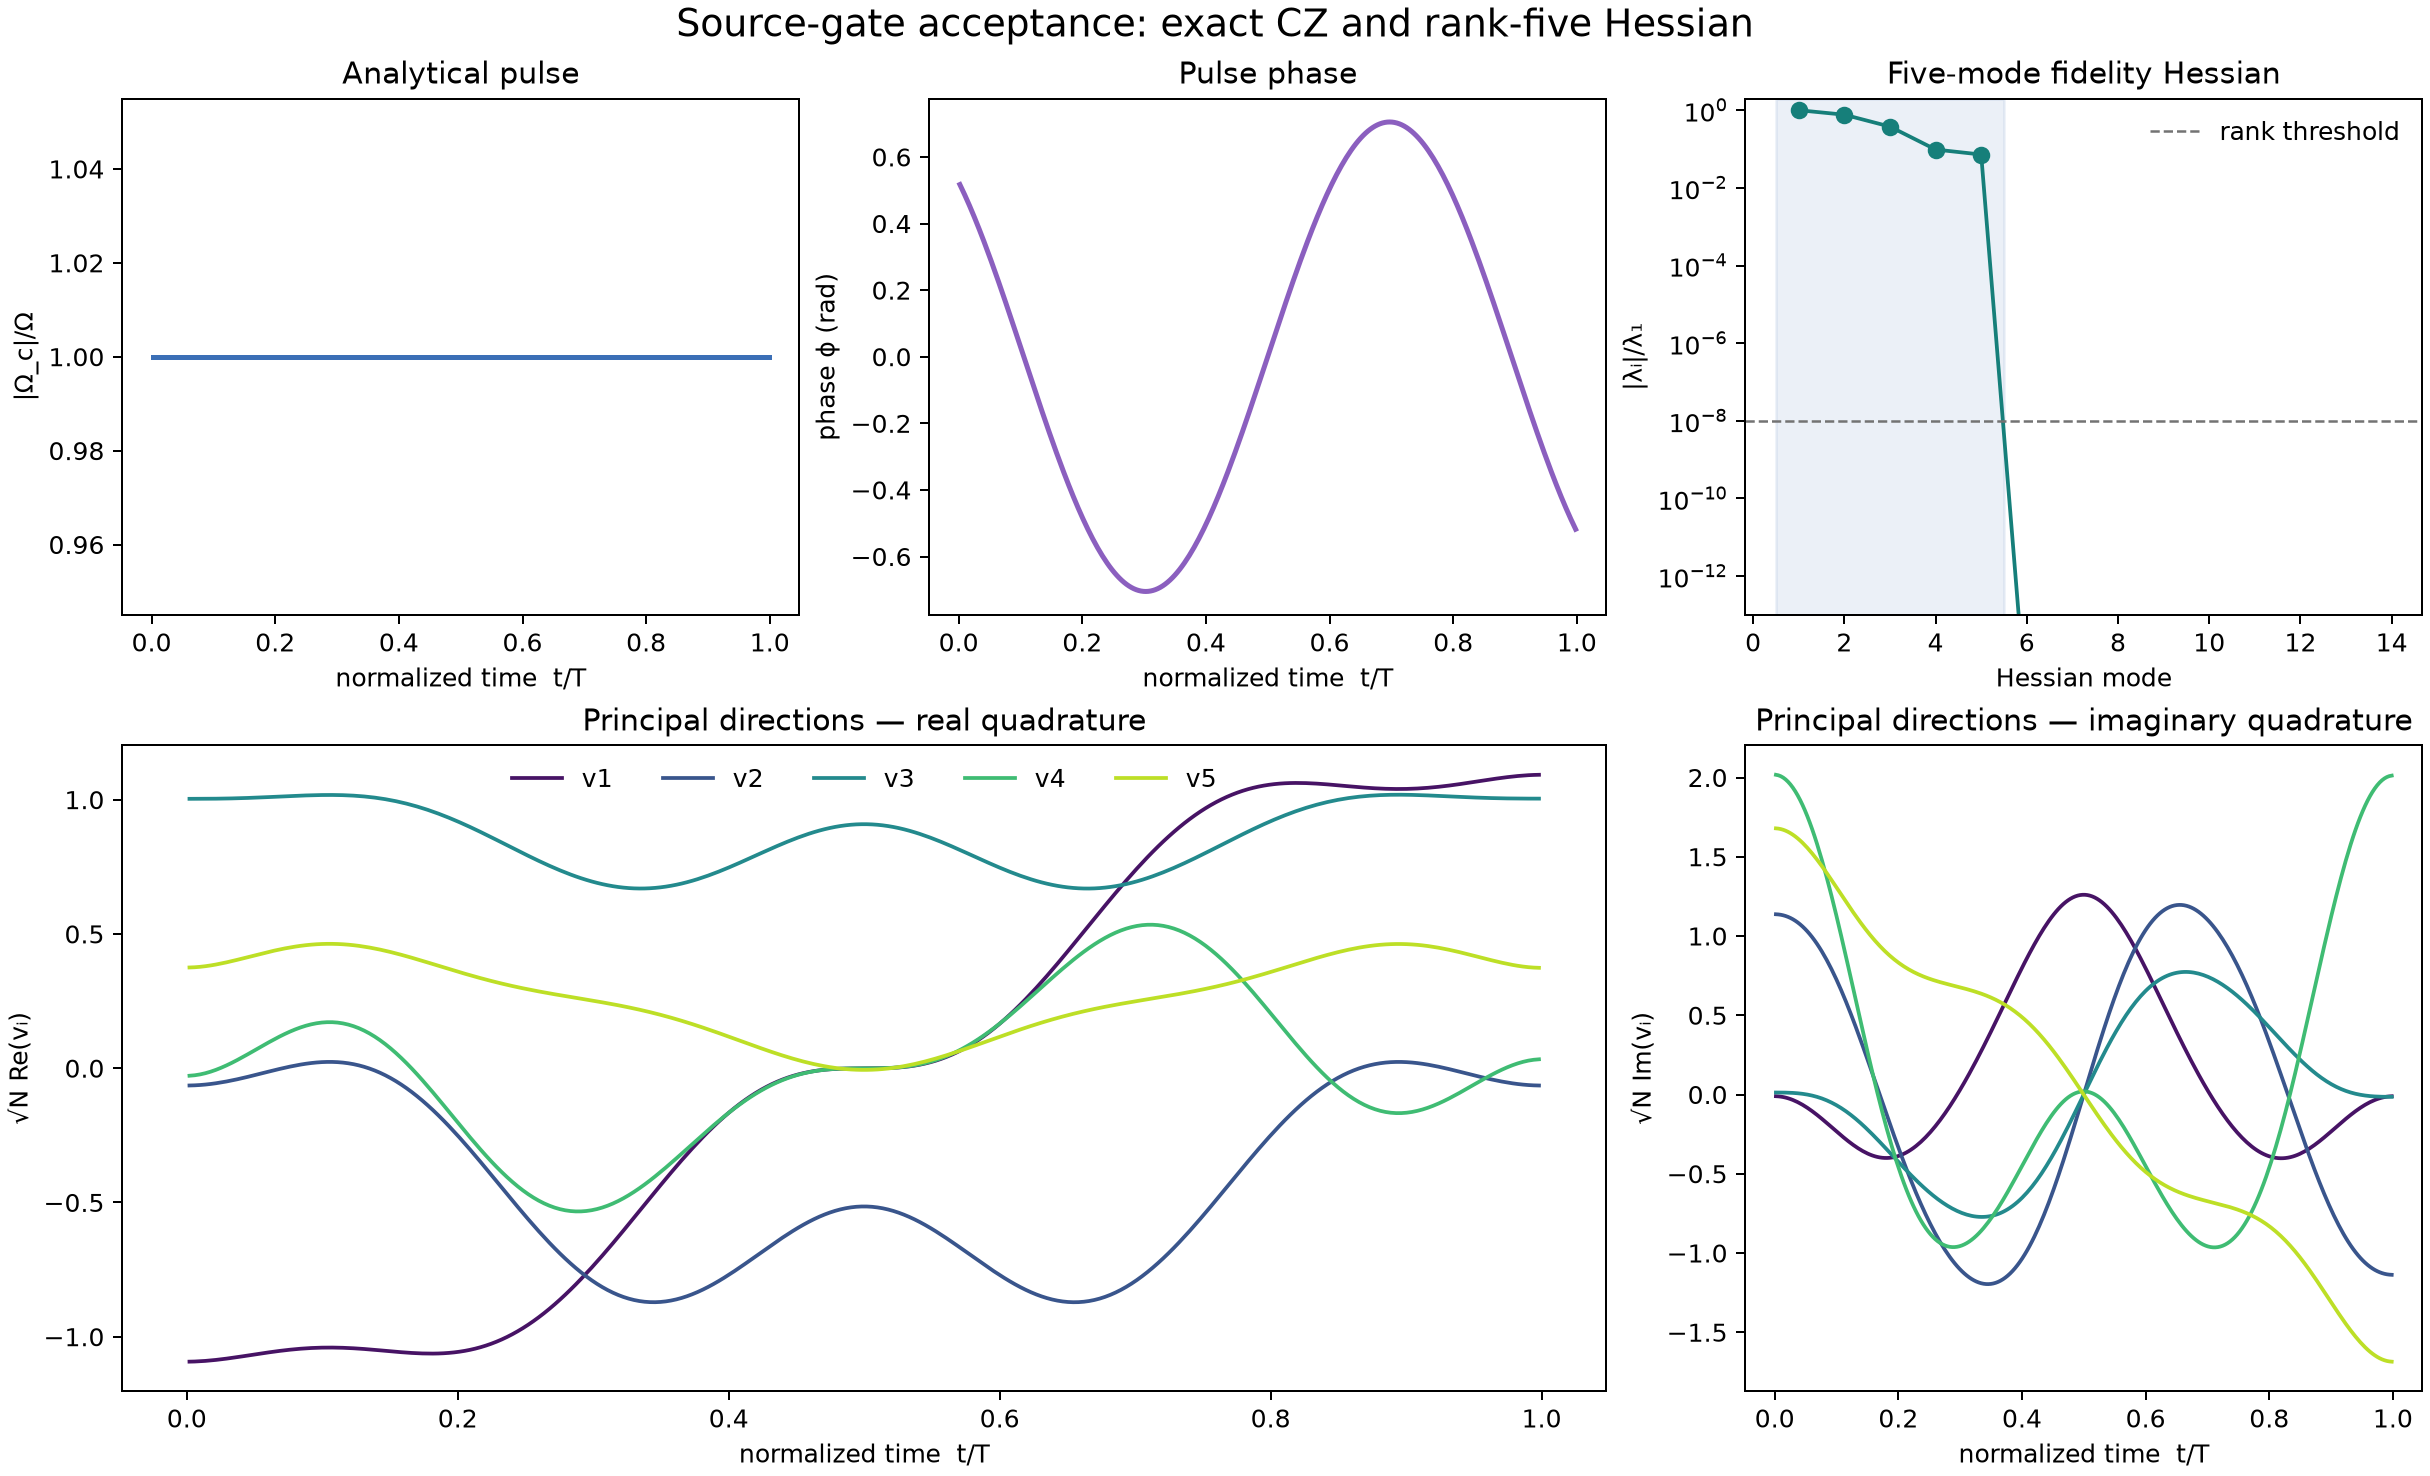
\includegraphics[width=\textwidth]{figs/fig01_baseline_hessian.png}
\caption{Nominal analytical pulse, leading Hessian spectrum, and the five
principal waveform directions.}
\end{figure}

\figReading{
The top-left panel shows that the pulse magnitude is constant:
$|\Om_c(t)|/\Om=1$.  The top-middle panel shows the phase modulation that
actually shapes the gate.  The top-right panel orders the Hessian eigenvalues
from largest to smallest and divides them by the largest eigenvalue.
Exactly five eigenvalues lie above the dashed rank threshold.

The lower panels show the real and imaginary quadratures of the five
eigenvectors.  Each curve is a direction in which the waveform can be
changed.  The optimizer scans coefficients along these shapes; it does not
independently scan all 512 time-bin coordinates.
}

\figMeaning{
The rounded analytical pulse gives $\infid=6.60\times10^{-6}$ and a
controlled-phase error of $1.94\times10^{-4}$ rad.  The ratio
$|\lambda_6|/\lambda_1=2.68\times10^{-16}$ confirms the intended rank-five
structure.  This figure is the acceptance test for the rest of the study.
}

\figCaution{
``Exact CZ'' in the figure title means exact numerical propagation of the
specified model, not zero mathematical error.  The published rounded pulse
constants leave the small residual error stated above.  Individual
eigenvectors can also change sign without changing their physical meaning;
only their span matters.
}

\clearpage
\subsection{Figure 2: representative optimization trajectories}

\begin{figure}[htbp]
\centering
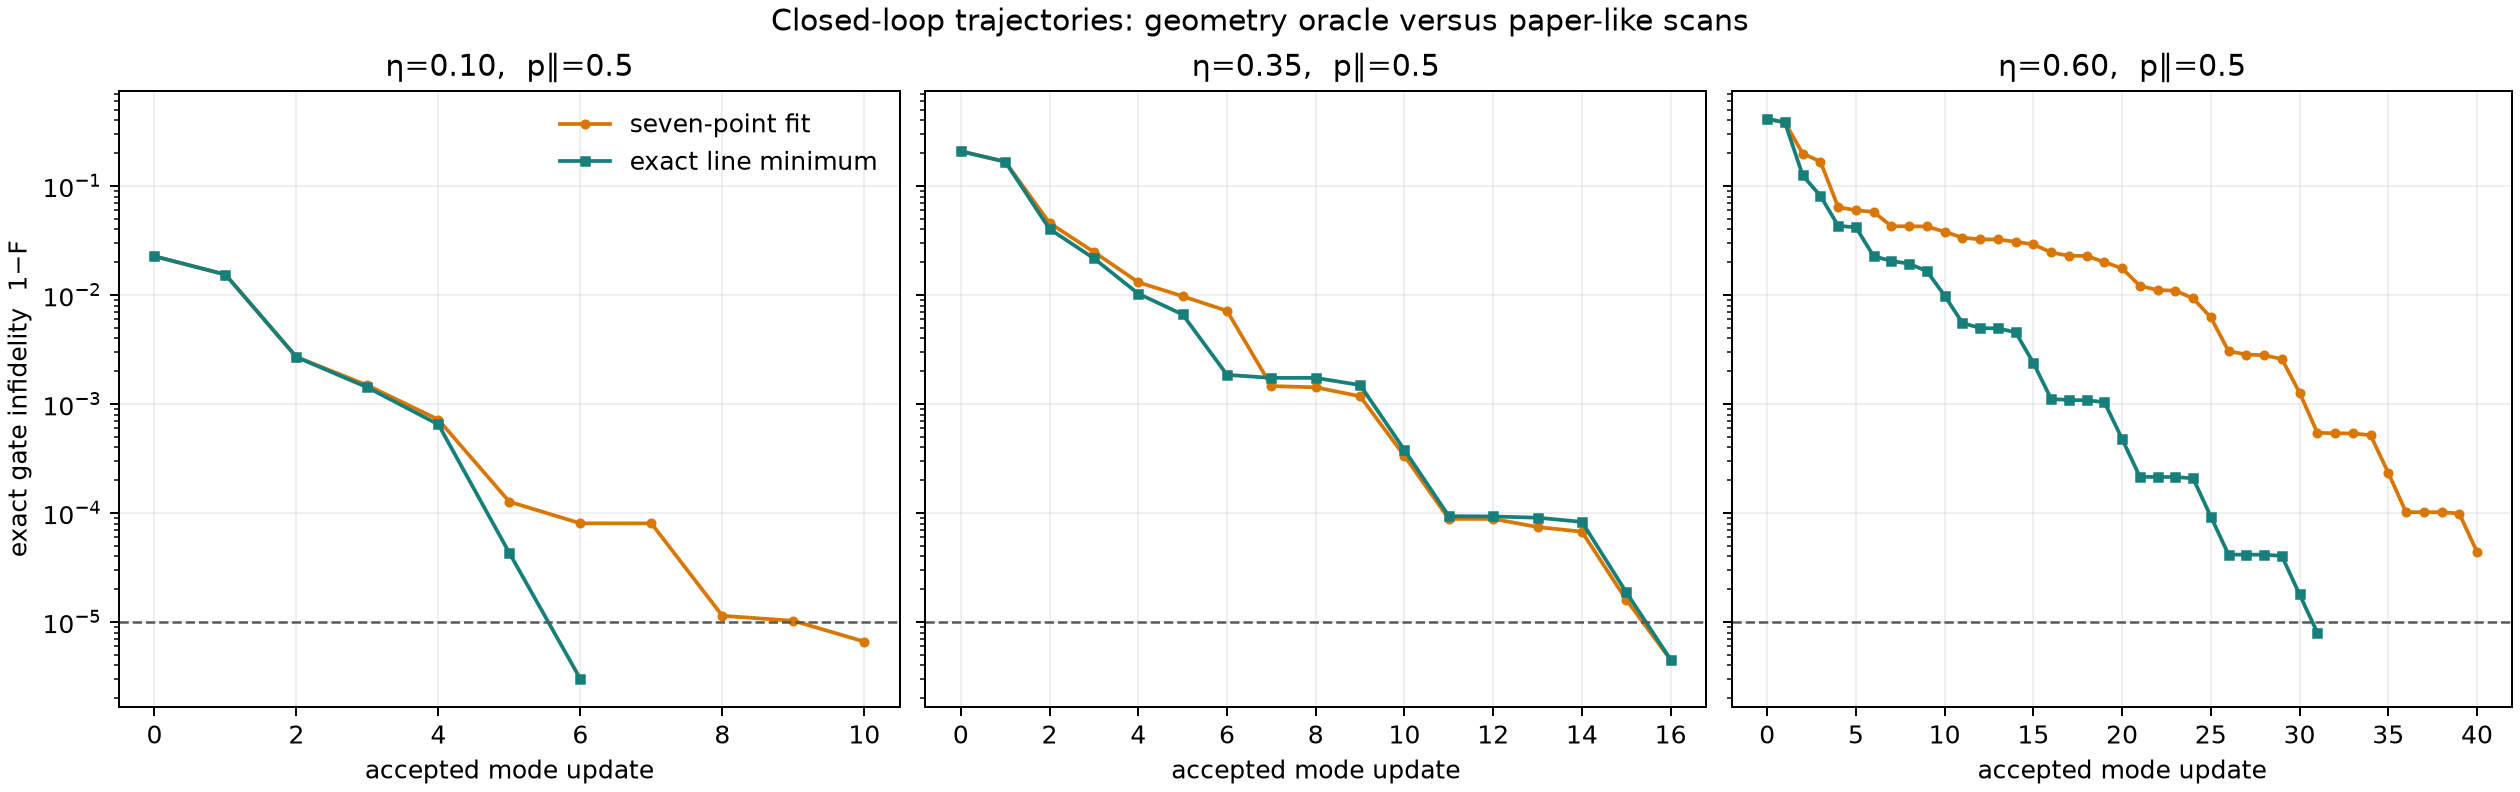
\includegraphics[width=\textwidth]{figs/fig02_trajectories.png}
\caption{Gate infidelity after every accepted mode update for mixed
distortions with $\pPar=0.5$.}
\end{figure}

\figReading{
The vertical axis is logarithmic, and the dashed horizontal line is the
success target $\infid=\target$.  The horizontal axis counts accepted
single-mode updates; five such updates are one complete cycle.

Orange circles use the experimentally plausible seven-point quadratic fit.
Green squares use an exact one-dimensional minimizer that has access to the
simulated fidelity function.  The green result is an oracle diagnostic, not
an experimentally available method.
}

\figMeaning{
At $\eta=0.10$ and $0.35$, both methods converge below the target.  At
$\eta=0.60$, the exact line minimizer still reaches
$\infid\simeq7.8\times10^{-6}$, while the seven-point fit stops near
$4.4\times10^{-5}$ in this representative seed.  Therefore this particular
failure is not proof that the five directions contain no useful descent
path.  It is largely a failure of the local quadratic line fit on a
non-parabolic landscape.
}

\figCaution{
This figure shows only one seed at each $\eta$.  The population success
fraction is in Figure~3.  Flat sections are also not necessarily a total
stall: a scanned direction may make little change before a later direction
produces a large drop.
}

\clearpage
\subsection{Figure 3: the closed-loop failure map}

\begin{figure}[htbp]
\centering
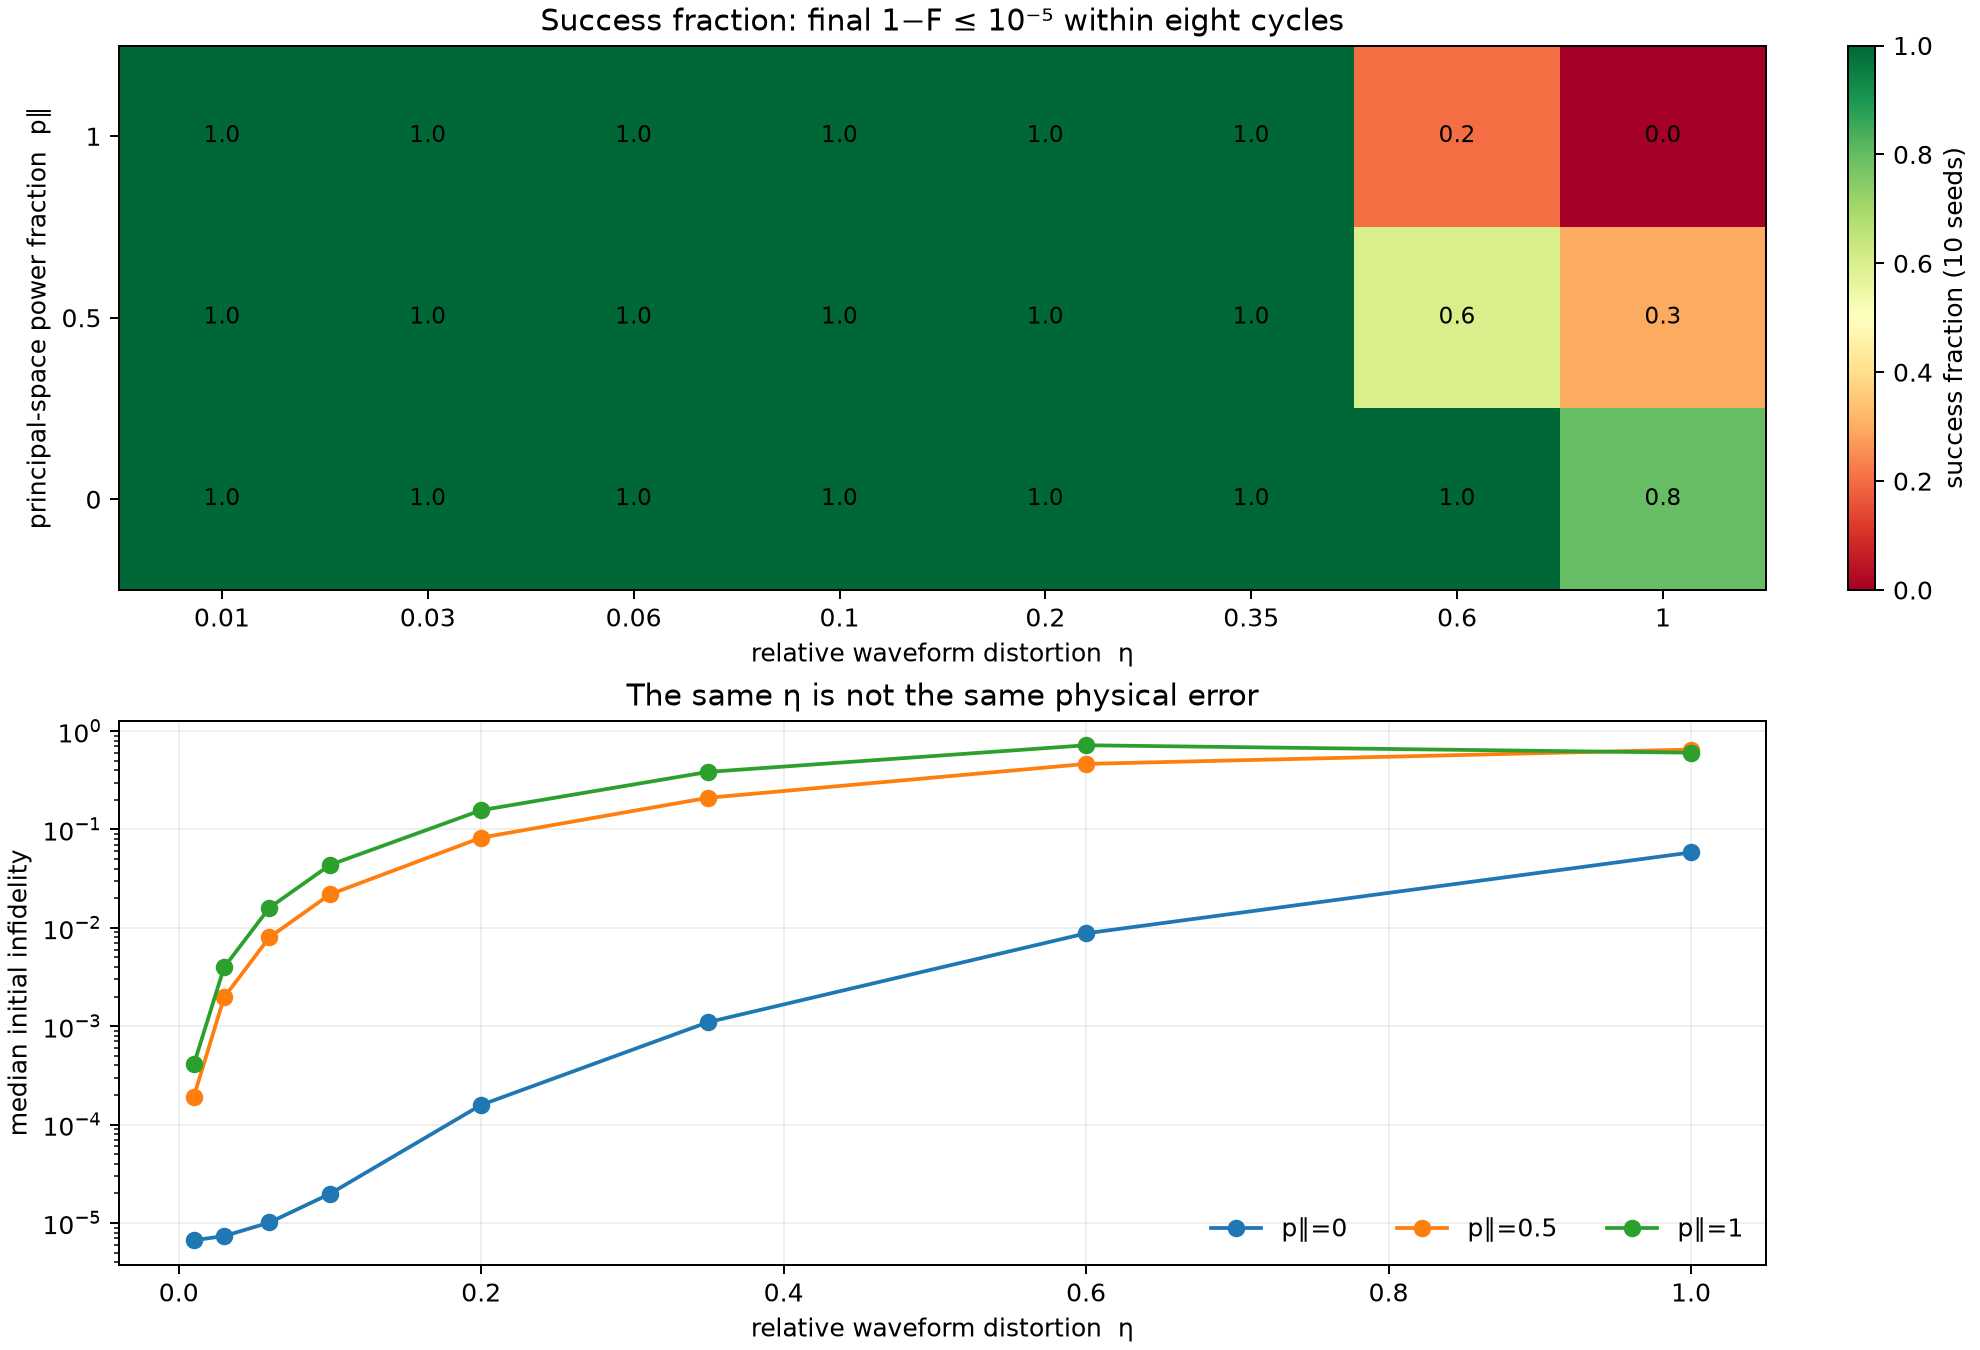
\includegraphics[width=\textwidth]{figs/fig03_failure_map.png}
\caption{Success fraction over ten smooth random distortions per cell, with
the corresponding median initial gate infidelity.}
\end{figure}

\figReading{
In the upper heat map, green means that all ten seeds reached the target and
red means that none did.  Columns increase the waveform norm $\eta$; rows
increase the fraction $\pPar$ initially placed in the five nominal Hessian
directions.

The lower panel is essential: it shows the median gate error before
optimization.  At the same $\eta$, a principal-space distortion can cause
orders of magnitude more gate error than a nominal-null-space distortion.
}

\figMeaning{
All three orientations succeed for all ten seeds through $\eta=0.35$.
At $\eta=0.60$, success is
\[
10/10\quad(\pPar=0),\qquad
6/10\quad(\pPar=0.5),\qquad
2/10\quad(\pPar=1).
\]
At $\eta=1$, the corresponding counts are $8/10$, $3/10$, and $0/10$.
Thus the first observed principal-rich failure boundary is bracketed by
$0.35<\eta\leq0.60$.
}

\figCaution{
It would be wrong to conclude that null-space errors are intrinsically
easier at equal physical gate error.  They look easier here at equal
waveform norm because the nominal Hessian does not see them at first order,
so their initial gate infidelity is much smaller.  Ten seeds give only an
exploratory boundary; for example, $6/10$ has a wide 95\% Wilson interval of
approximately $0.31$--$0.83$.
}

\clearpage
\subsection{Figure 4: when the quadratic Hessian model stops being accurate}

\begin{figure}[htbp]
\centering
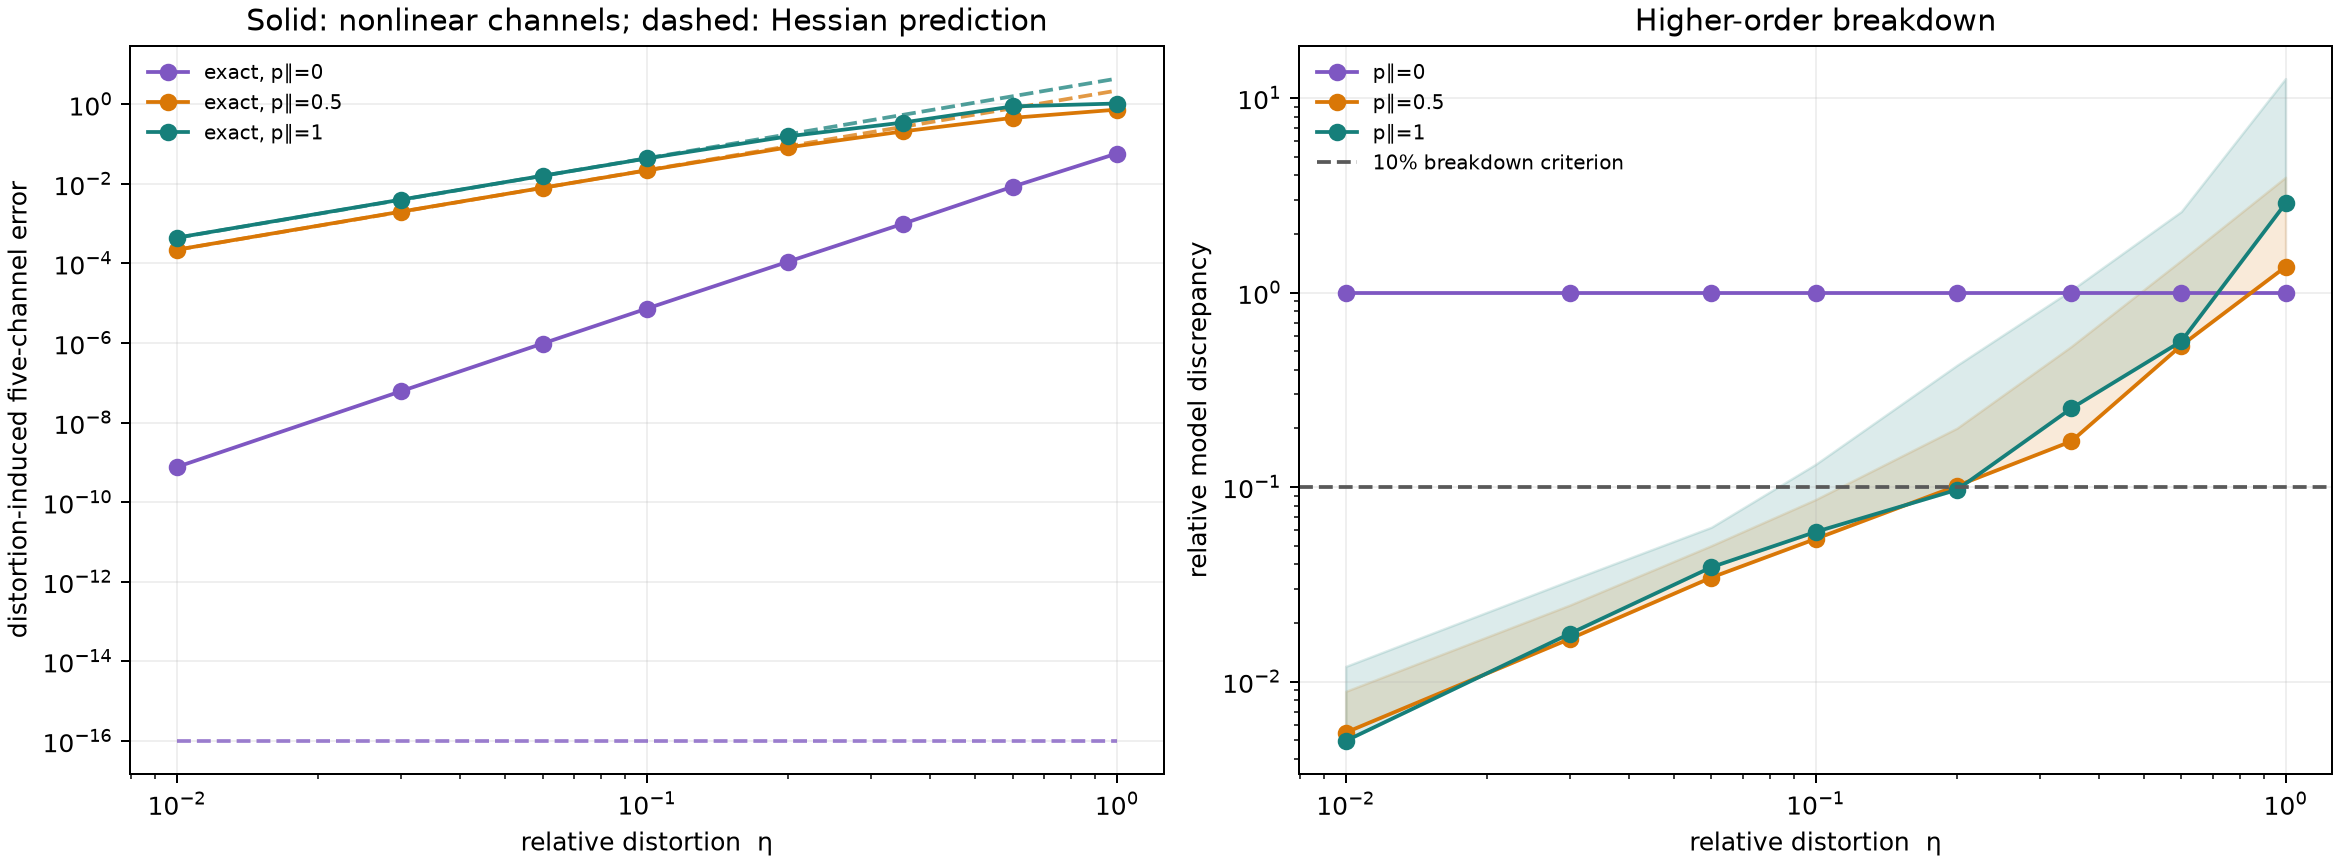
\includegraphics[width=\textwidth]{figs/fig04_quadratic_breakdown.png}
\caption{Nonlinear five-channel error compared with the leading Hessian
prediction, and their relative discrepancy.}
\end{figure}

\figReading{
In the left panel, solid curves are obtained by propagating the distorted
pulse and evaluating the nonlinear leakage/phase channels.  Dashed curves
are the prediction
\[
\frac{1}{2}\dOm^{\mathsf T}\Hess\dOm.
\]
The right panel plots their relative difference.  The horizontal dashed
line marks the chosen 10\% breakdown criterion.  Shading extends from the
median to the 90th percentile across seeds.
}

\figMeaning{
For $\pPar=0.5$, the median discrepancy is about 5.4\% at $\eta=0.10$,
10.1\% at $\eta=0.20$, and 53.4\% at $\eta=0.60$.  Therefore the
small-distortion expansion starts losing quantitative accuracy well before
the success fraction collapses.  The optimizer can tolerate some model
error, but not unlimited model error.
}

\figCaution{
For $\pPar=0$, the Hessian prediction is zero by construction.  The exact
higher-order channel error is nonzero, so the relative discrepancy is
essentially one at every $\eta$.  This does \emph{not} mean a tiny null-space
distortion is catastrophic; the left panel shows that its absolute error is
very small at small $\eta$.  Also, the plotted ``exact'' channel metric is
baseline-relative and is not the raw total gate infidelity.
}

\clearpage
\subsection{Figure 5: rotation of the locally sensitive subspace}

\begin{figure}[htbp]
\centering
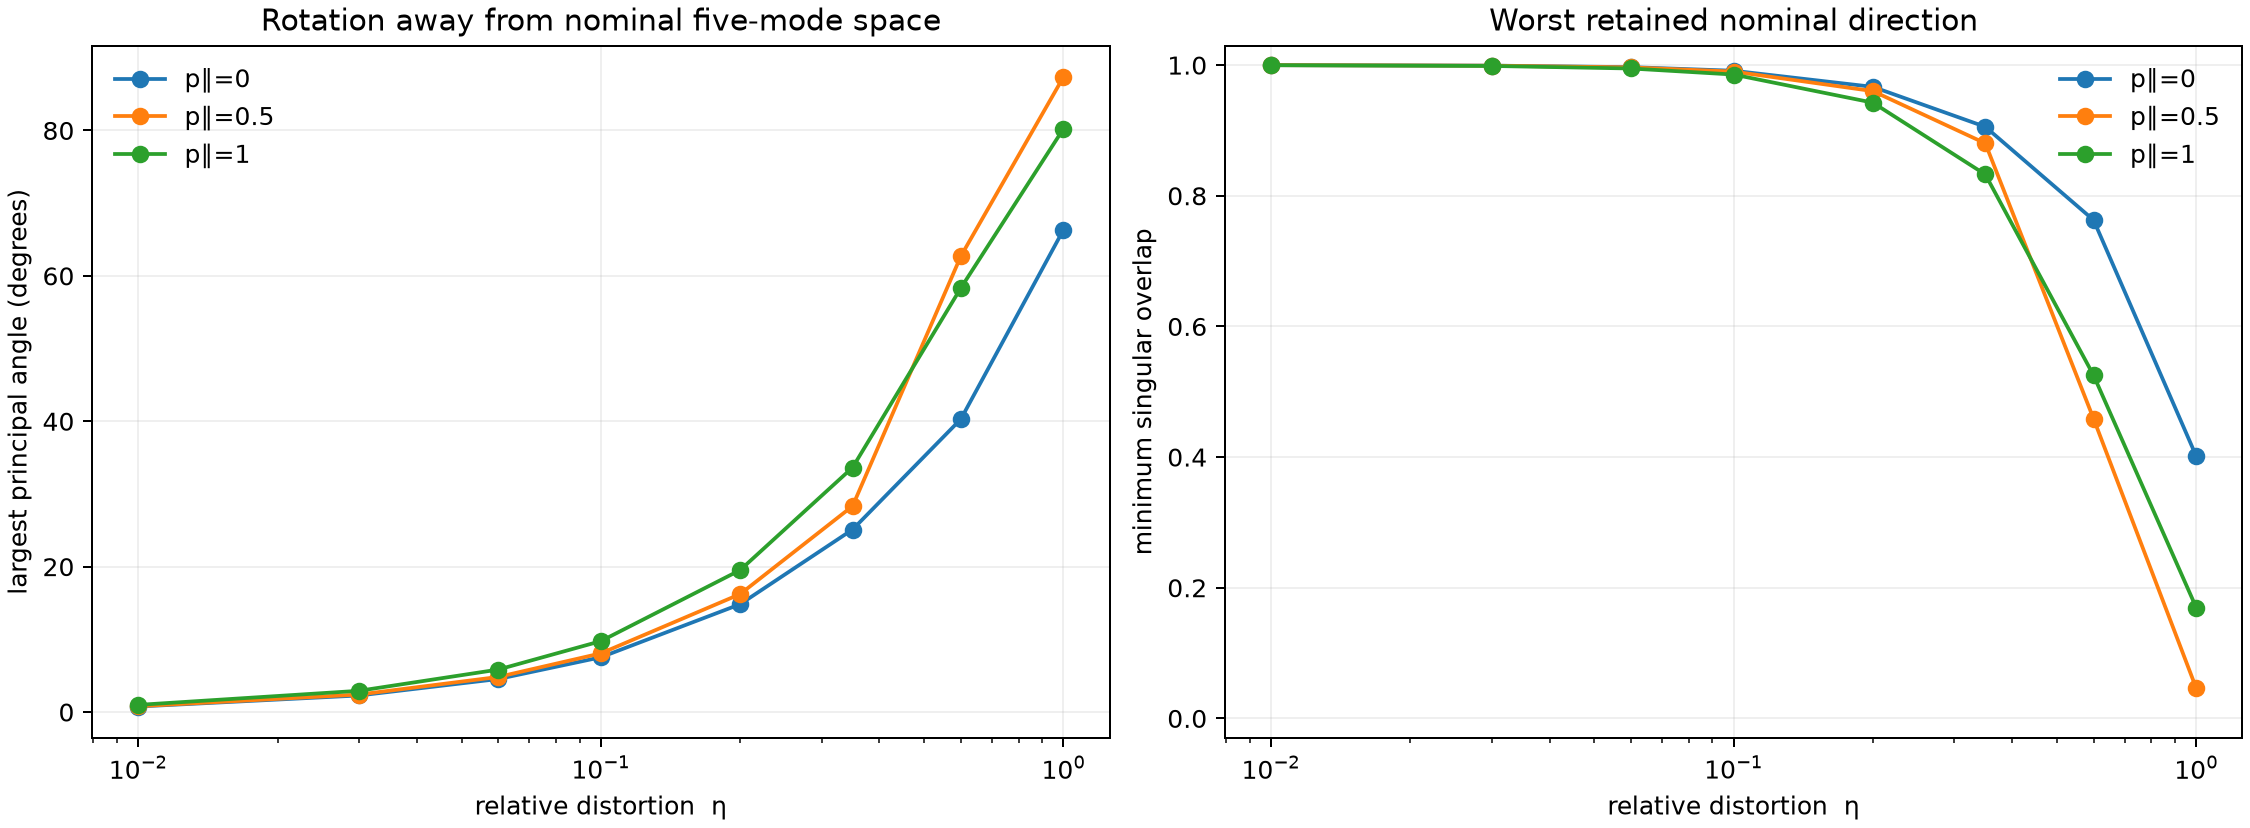
\includegraphics[width=\textwidth]{figs/fig05_subspace_rotation.png}
\caption{Geometric comparison of the nominal and distorted-pulse
five-dimensional Hessian subspaces.}
\end{figure}

\figReading{
At each distorted waveform, a new local five-mode Hessian is calculated.
The left panel shows the largest principal angle between this local subspace
and the nominal one.  Zero degrees means perfect alignment; 90 degrees means
that at least one local sensitive direction is orthogonal to its best
nominal counterpart.

The right panel shows the smallest singular overlap.  One means that every
local direction is retained well; zero means that one useful direction has
been almost completely lost by the fixed nominal scan space.
}

\figMeaning{
At $\eta=0.35$, the largest angle is only about
$25^\circ$--$34^\circ$, and every scan cell succeeds.  At $\eta=0.60$, it
grows to about $40^\circ$--$63^\circ$ and the principal-rich success
fraction becomes seed-dependent.  For the mixed case at $\eta=1$, the angle
is $87.4^\circ$ and the worst overlap is only 0.046.
}

\figCaution{
The local Hessian still has five active modes; the issue is rotation, not a
change from rank five to another rank.  The correlation between rotation and
failure is strong in this scan, but it is a diagnostic rather than a formal
proof of causation.
}

\clearpage
\subsection{Figure 6: which error channels remain after calibration?}

\begin{figure}[htbp]
\centering
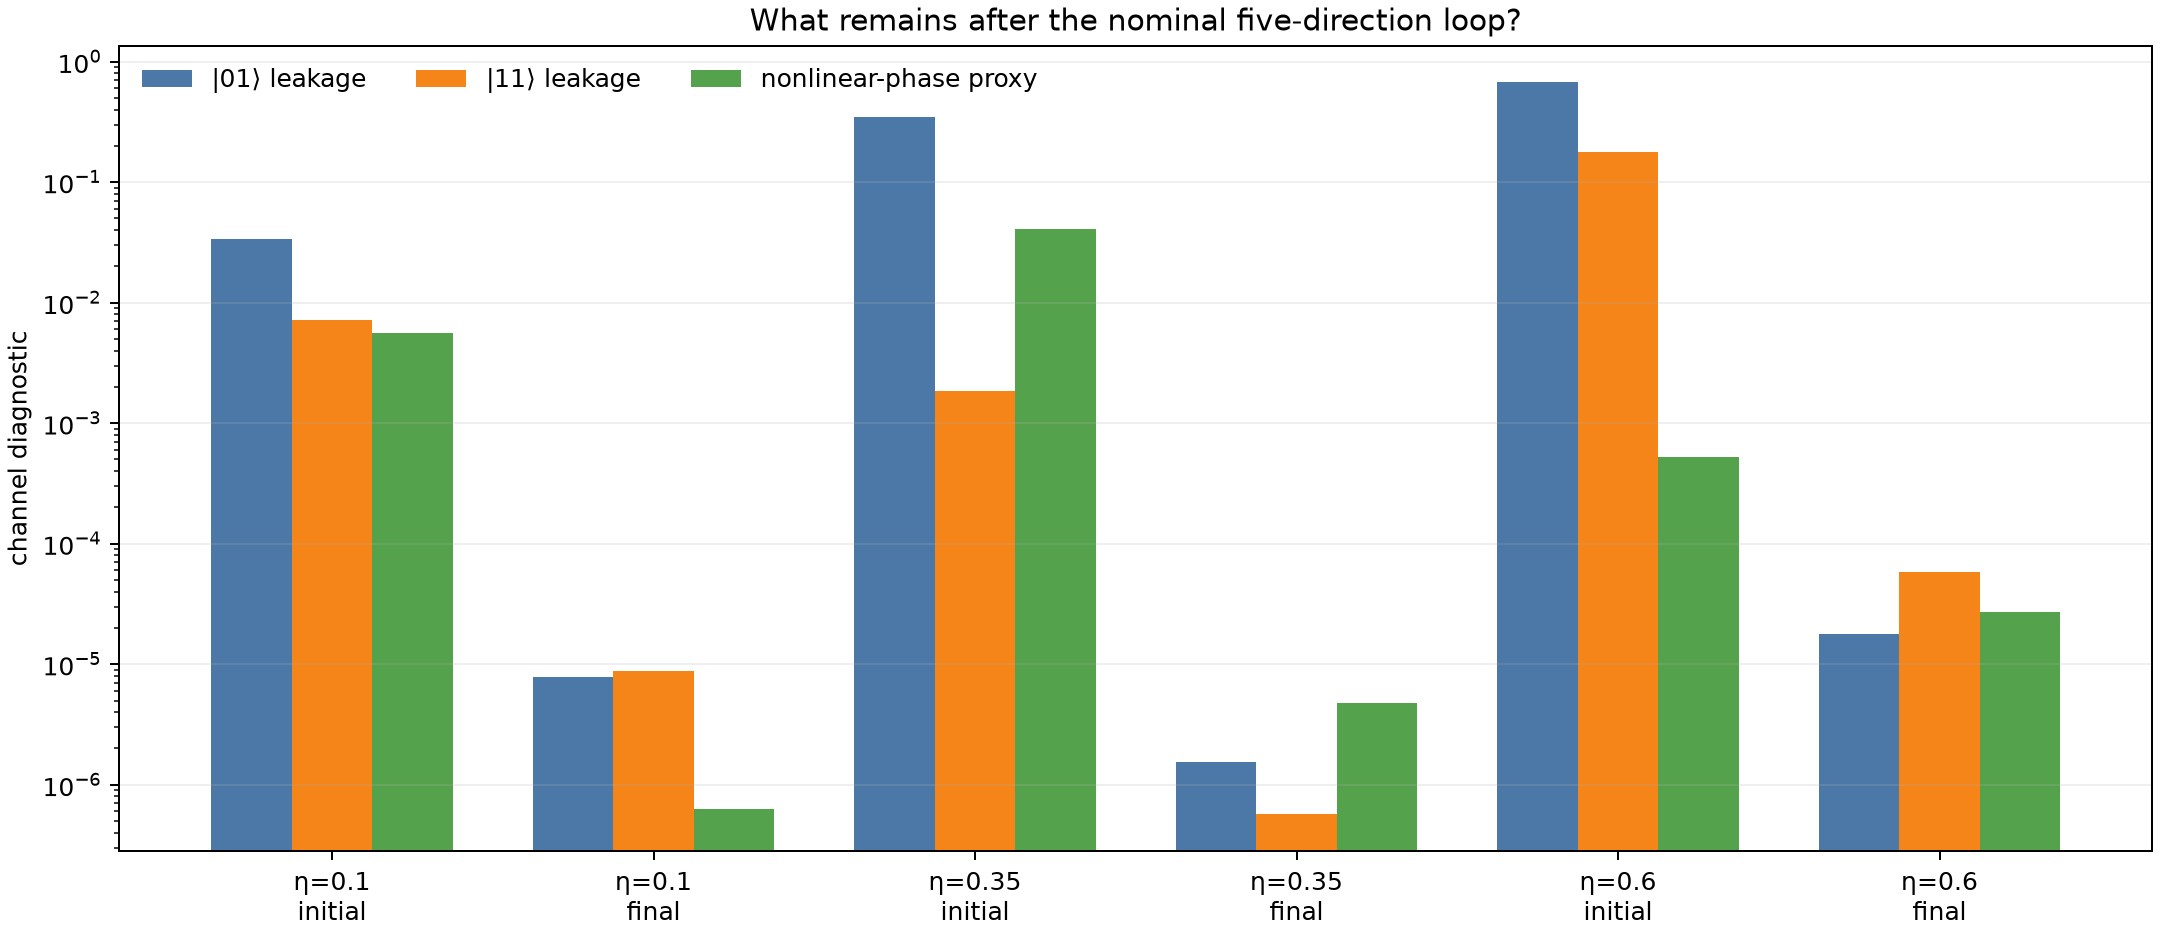
\includegraphics[width=\textwidth]{figs/fig06_channel_decomposition.png}
\caption{Initial and final leakage/phase diagnostics for one mixed seed at
three distortion strengths.}
\end{figure}

\figReading{
Each $\eta$ has an initial group and a final group.  Blue is leakage from
the $|01\rangle$ sector, orange is leakage from the $|11\rangle$ sector,
and green is a nonlinear-phase proxy $\delta\theta^2/5$.  The vertical axis
is logarithmic, so a one-decade drop is a factor of ten.
}

\figMeaning{
At $\eta=0.10$ and $0.35$, the loop suppresses all three diagnostics to
roughly the target scale or below.  For the failed $\eta=0.60$ trajectory,
the final values are approximately
\[
P_{\mathrm{leak},01}=1.79\times10^{-5},\quad
P_{\mathrm{leak},11}=5.85\times10^{-5},\quad
\delta\theta^2/5=2.71\times10^{-5}.
\]
The plateau is therefore a mixture of leakage and phase error, not a single
bad phase coefficient.
}

\figCaution{
These bars are channel diagnostics, not three exactly additive pieces of
the total infidelity.  Their fidelity weights differ, and higher-order cross
terms remain.  Compare orders of magnitude and before/after suppression,
not the sum of bar heights.
}

\clearpage
\subsection{Figure 7: failure caused by noisy fidelity estimates}

\begin{figure}[htbp]
\centering
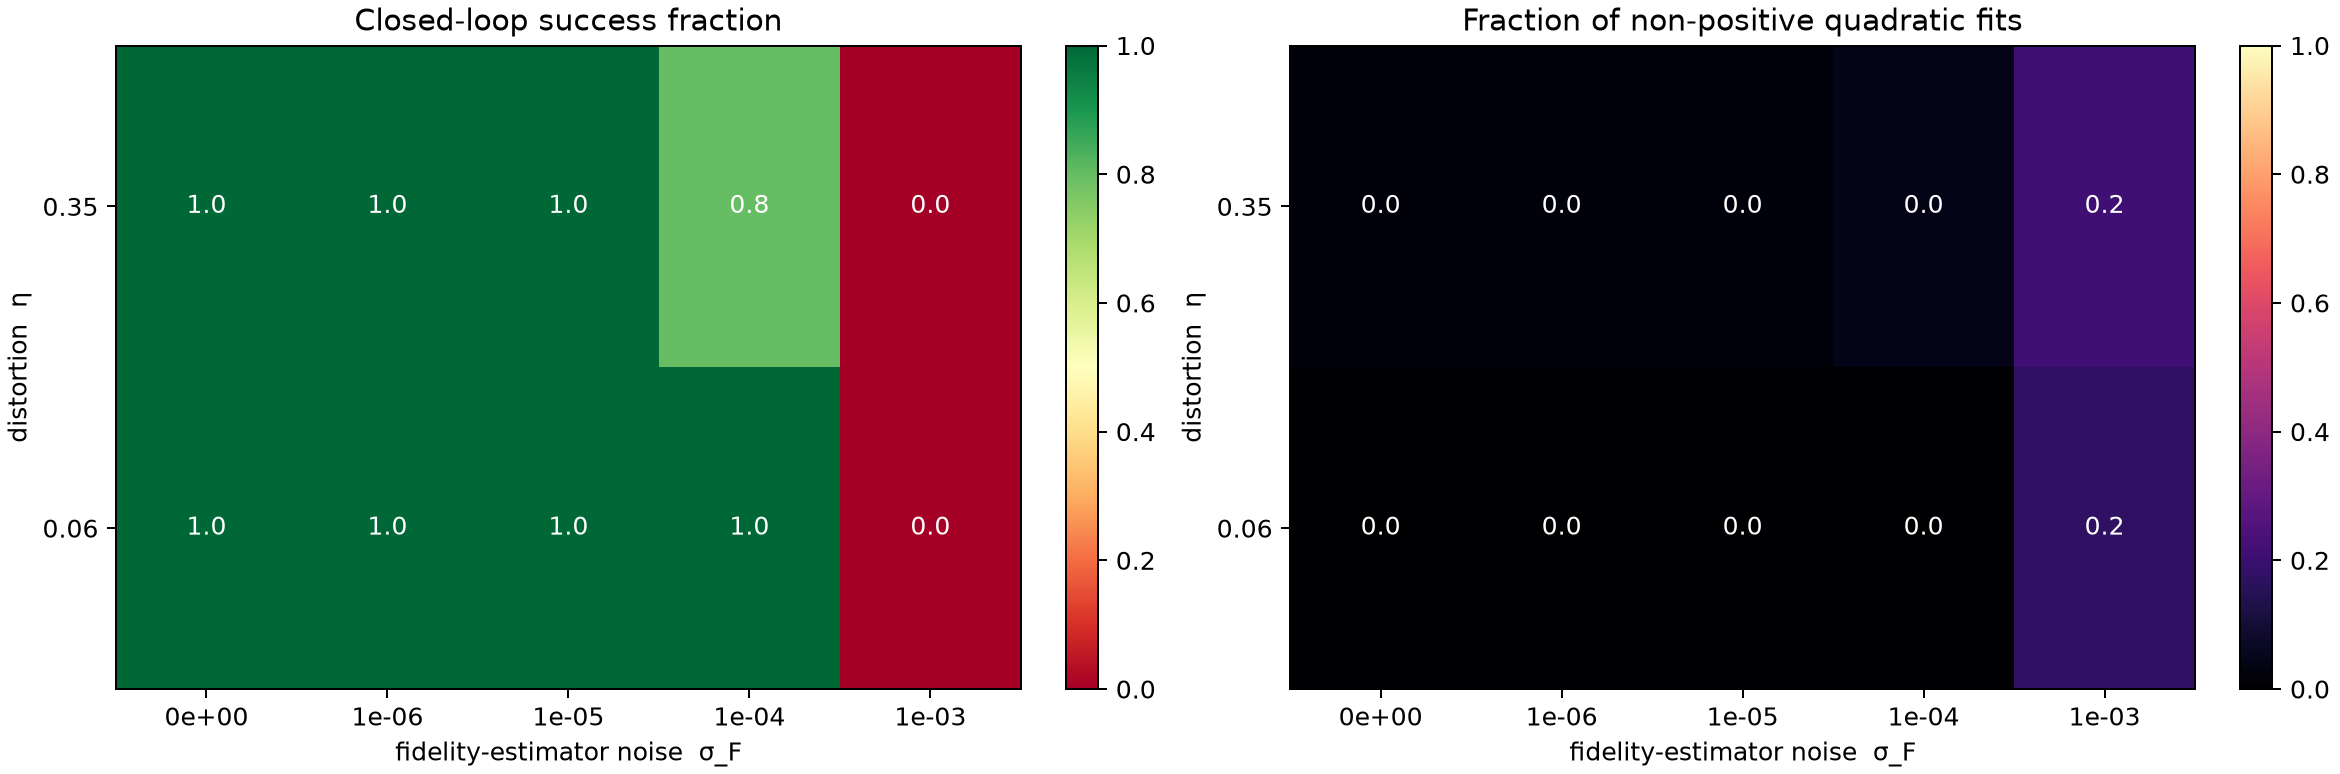
\includegraphics[width=\textwidth]{figs/fig07_noise_conditioning.png}
\caption{Success and quadratic-fit stability versus additive scalar
fidelity-estimator noise.}
\end{figure}

\figReading{
The left heat map is the success fraction over ten seeds.  The right heat
map is the median fraction of line scans whose fitted quadratic curvature is
non-positive.  A non-positive fitted curvature is a warning that noise has
overwhelmed the local convex signal or that the sampled line is strongly
non-quadratic.
}

\figMeaning{
For $\eta=0.06$, all seeds succeed through $\sigma_F=10^{-4}$ and none
succeeds at $10^{-3}$.  For $\eta=0.35$, success is $8/10$ at $10^{-4}$
and $0/10$ at $10^{-3}$.  Thus this estimator's noise boundary lies between
$10^{-4}$ and $10^{-3}$ in absolute fidelity units.
}

\figCaution{
The noise is independent additive Gaussian noise on a scalar fidelity
estimate.  It is not a shot-resolved randomized-benchmarking or survival
probability model.  The threshold therefore diagnoses numerical
conditioning of this seven-point rule; it is not a universal experimental
shot-count requirement.  The displayed value 0.2 at $\sigma_F=10^{-3}$ is
rounded from medians near 0.18--0.21.
}

\clearpage
\subsection{Figure 8: six ``weird'' or ill-conditioned controls}

\begin{figure}[htbp]
\centering
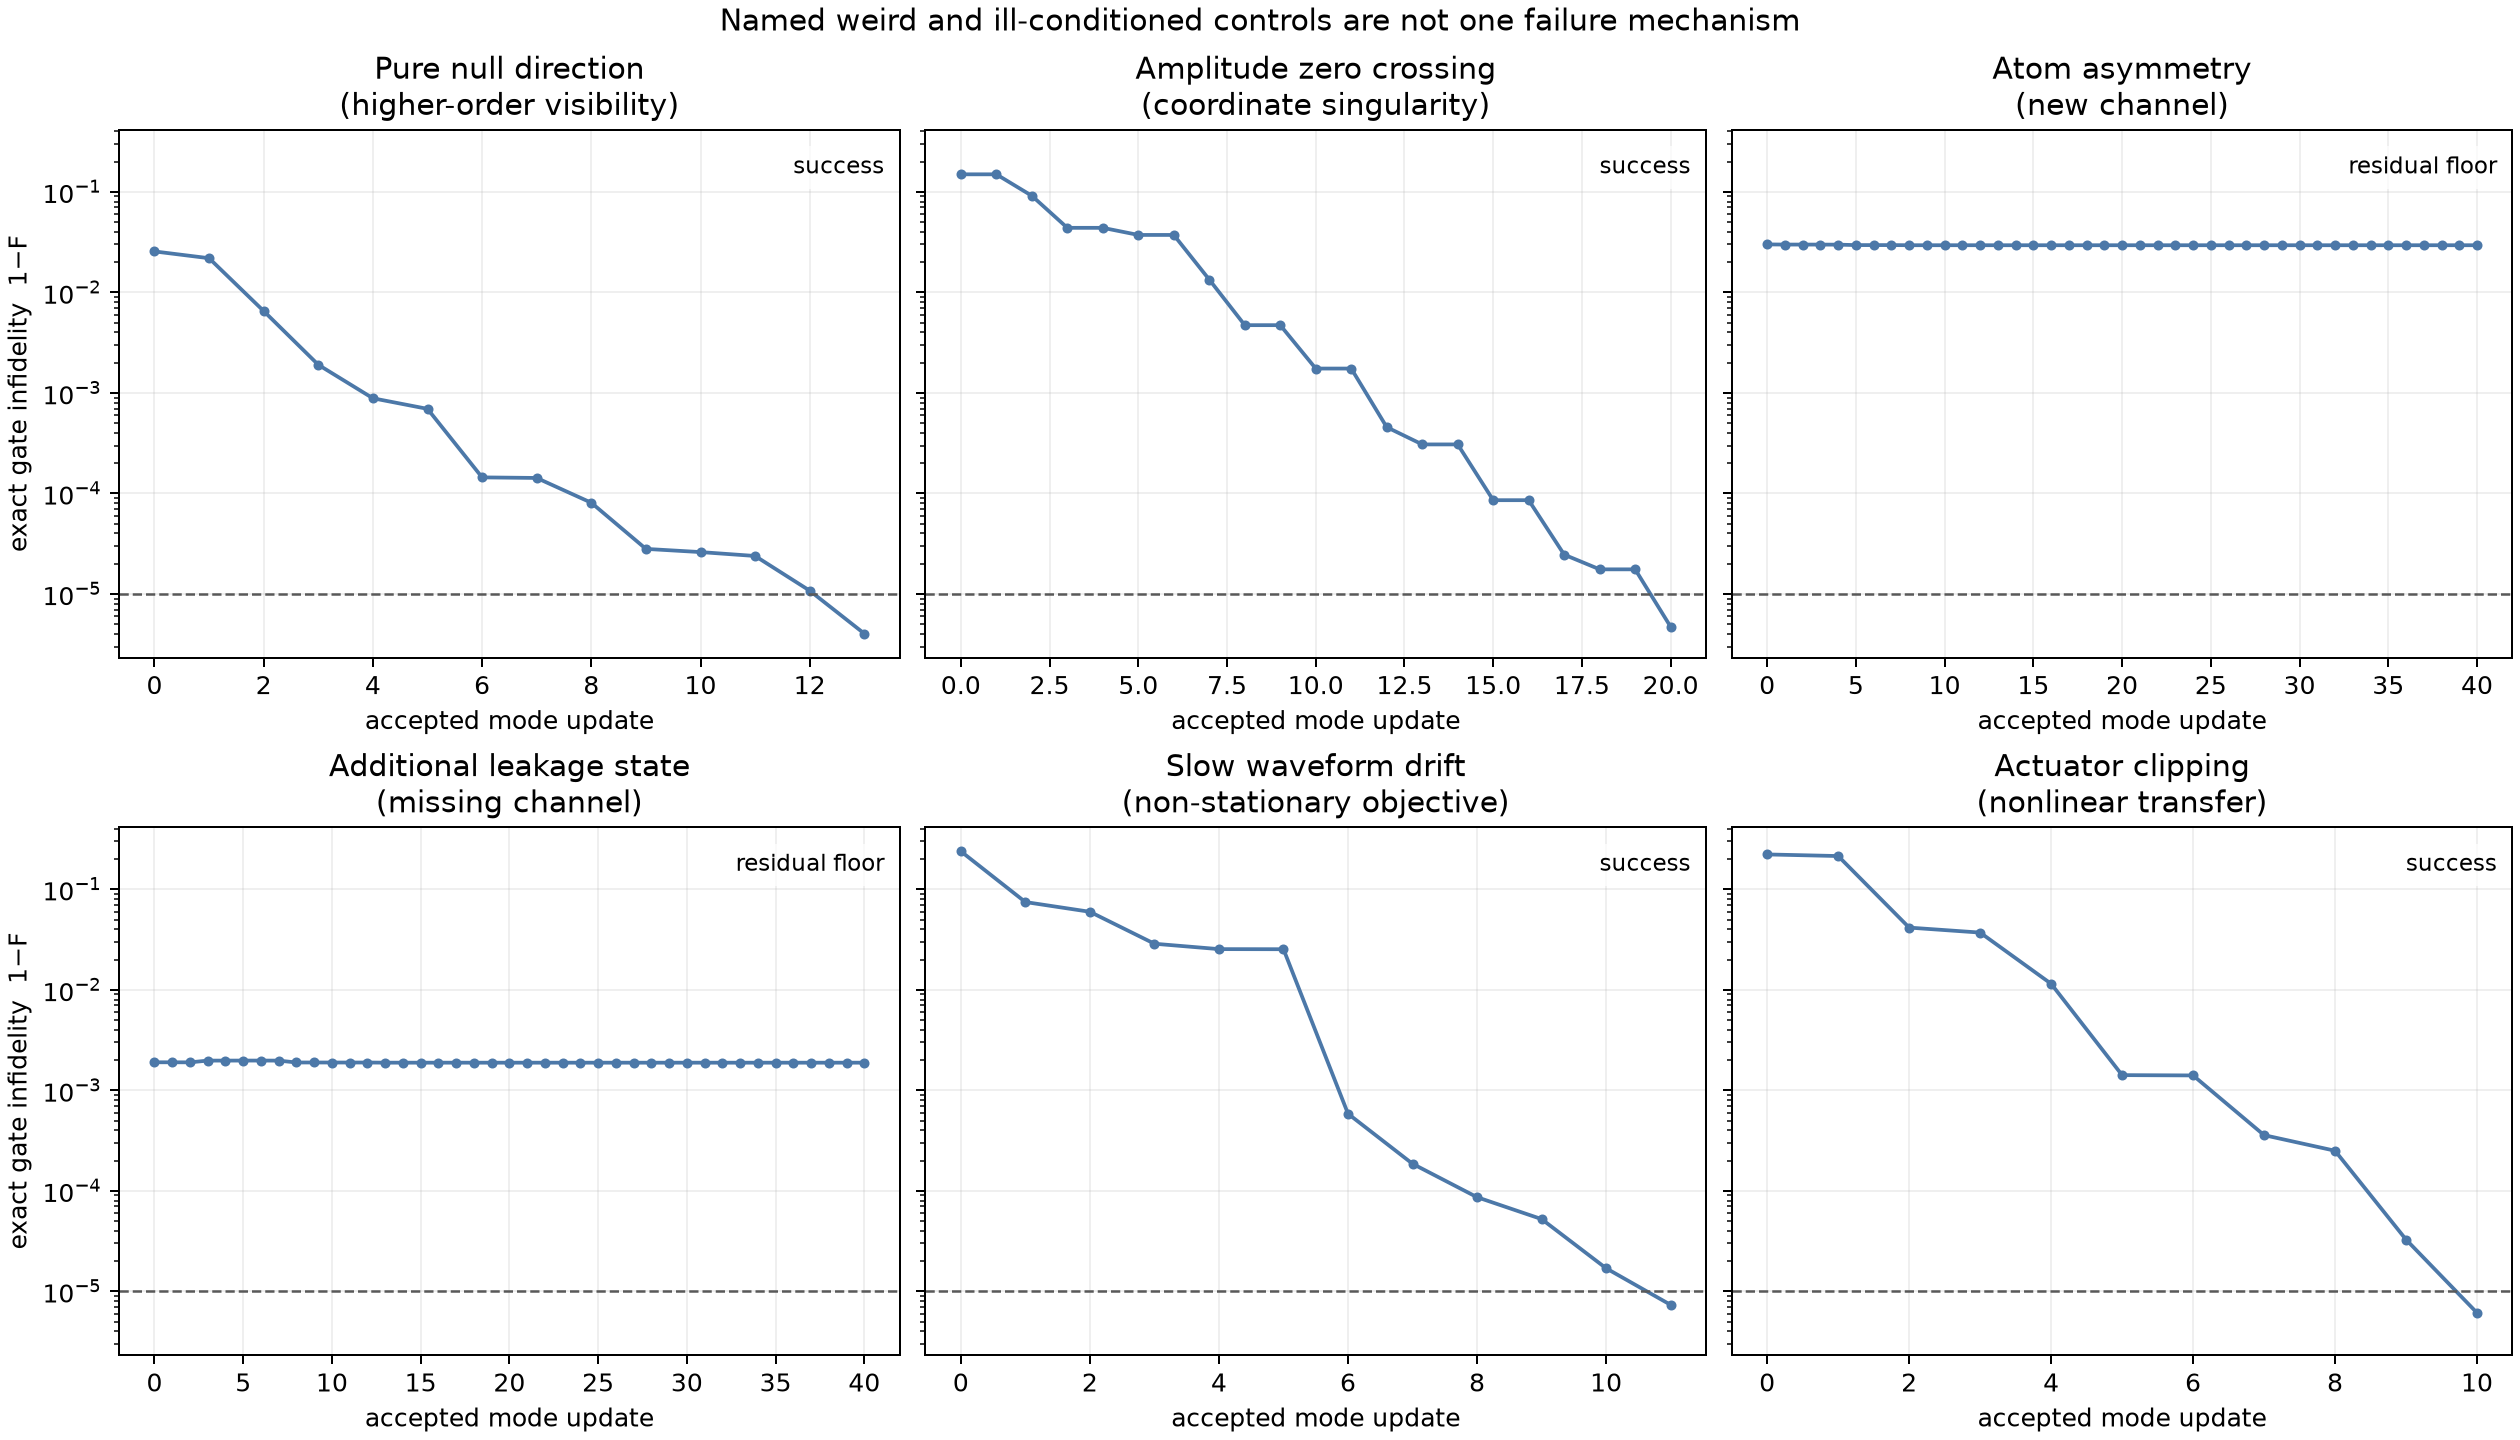
\includegraphics[width=\textwidth]{figs/fig08_pathology_gallery.png}
\caption{Infidelity trajectories for six explicitly defined stress tests.}
\end{figure}

\figReading{
Every panel uses the same logarithmic infidelity axis and the same dashed
success target.  ``Residual floor'' means that eight cycles did not cross
the target; ``success'' means that the trajectory did.
}

\figMeaning{
\begin{itemize}
\item \textbf{Pure null direction:} a large $\eta=0.60$ distortion that is
  invisible to the nominal Hessian at first order still converges to
  $4.04\times10^{-6}$ because higher-order dynamics make it visible.
\item \textbf{Amplitude zero crossing:} a localized 105\% cancellation of
  the complex pulse converges to $4.72\times10^{-6}$.  Cartesian
  quadratures remain regular when the amplitude crosses zero.
\item \textbf{Atom asymmetry:} opposite differential drives on the two
  single-excitation sectors leave a floor near $2.95\times10^{-2}$.
\item \textbf{Additional leakage state:} coupling one sector to a new state
  leaves a floor near $1.88\times10^{-3}$.
\item \textbf{Slow waveform drift:} a null-like drift of norm
  $\eta=0.02$ per cycle is tracked successfully, reaching
  $7.35\times10^{-6}$.
\item \textbf{Actuator clipping:} a nonlinear amplitude cap at
  $1.05\Om$ is also compensated in this case, reaching
  $6.12\times10^{-6}$.
\end{itemize}
}

\figCaution{
These are single representative probes, not probability distributions.
The conclusion is not that drift and clipping are always safe.  It is that
``weird-looking'' control coordinates alone do not determine failure.
The two clear floors arise from missing physical channels that the fixed
five-direction space was never designed to control.
}

\clearpage
\subsection{Figure 9: in-span detuning versus a new leakage channel}

\begin{figure}[htbp]
\centering
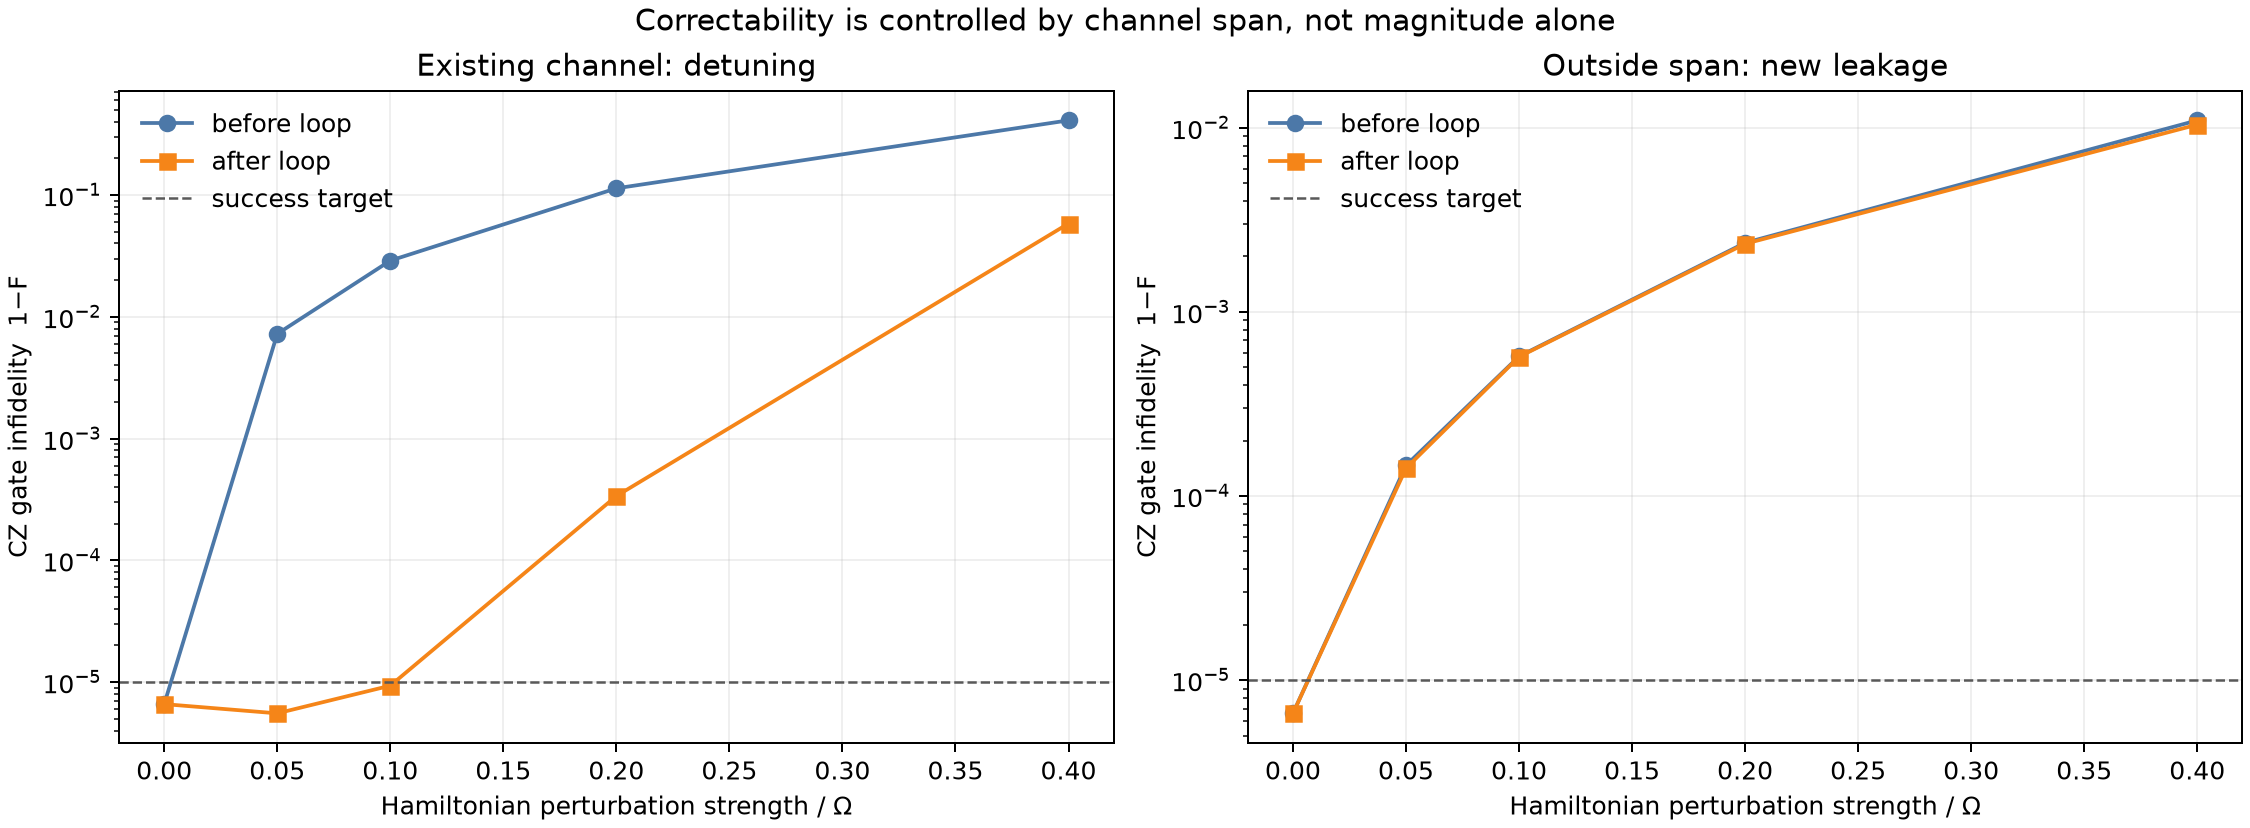
\includegraphics[width=\textwidth]{figs/fig09_hamiltonian_channels.png}
\caption{Gate infidelity before and after the loop for two Hamiltonian-error
families.}
\end{figure}

\figReading{
Blue circles show the gate before calibration and orange squares show it
after calibration.  The horizontal dashed line is the target.  The left
panel adds a detuning term that modifies the already existing dynamical
channels.  The right panel couples the system to an additional leakage
state, creating a response absent from the nominal five-channel model.
}

\figMeaning{
A detuning of $0.10\Om$ is corrected from
$\infid=2.89\times10^{-2}$ to $9.35\times10^{-6}$.  At $0.20\Om$, the loop
still improves the gate strongly but stops at $3.37\times10^{-4}$.

By contrast, a new leakage coupling of only $0.05\Om$ starts with a much
smaller error but remains at $1.41\times10^{-4}$ after calibration.  This is
the central physical message: correctability depends on whether the error
lies in the response span of the calibrated directions, not only on the
raw perturbation magnitude.
}

\figCaution{
``Existing channel'' does not mean that arbitrary detuning is always
correctable.  The fixed scan succeeds only through the tested
$0.10\Om$ point under the strict $\target$ criterion.  Correcting a new
leakage channel would generally require measuring that channel and enlarging
the Hessian/scan space.
}

\section{How the figures fit together}

The figures support the following diagnostic sequence:
\begin{enumerate}
\item Use Figure~1 to verify that the nominal gate and rank-five construction
  are correct.
\item Use Figure~3 to locate the empirical failure region.
\item Use Figure~4 to ask whether the small-distortion expansion has failed.
\item Use Figure~5 to ask whether the locally sensitive subspace has rotated
  away from the fixed nominal directions.
\item Use Figure~2 to distinguish a poor seven-point fit from the absence of
  a useful descent path.
\item Use Figure~6 to identify which nominal channels remain.
\item Use Figure~7 to test whether estimator noise makes line curvature
  unresolvable.
\item Use Figures~8 and 9 to test whether the device contains a genuinely new
  physical channel.
\end{enumerate}

The practical lesson is that there is no single universal ``maximum
$\|\dOm\|$''.  A useful failure criterion must report at least the waveform
norm, the initial physical infidelity, the orientation relative to the
nominal Hessian, the rotation of the local subspace, estimator noise, and
whether new Hamiltonian channels are present.

\section{Scope and reproducibility}

This is an exploratory perfect-blockade unitary study with ten random seeds
per core scan cell.  It does not include spontaneous decay, Doppler noise,
finite blockade, or the full four-level experimental ytterbium model.
The seven-point fit rule is an explicit extension choice because the paper
does not publish all experimental scan-width and fitting details.

The paper is available at
\url{https://arxiv.org/pdf/2606.05060v1}.
The complete calculation is implemented in
\path{robustness/comparison/code/hessian_loop_failure_map.py}.
The numerical tables are in the run's \path{data/} directory, and the
figures are in \path{figs/}.

\end{document}
